\documentclass{article}
\usepackage{geometry}
\geometry{legalpaper, margin=1in}
\usepackage[utf8]{inputenc}
\usepackage{hyperref}
\usepackage{graphicx}
\hypersetup{
    colorlinks=true,
    linkcolor=blue,
    filecolor=magenta,
    urlcolor=cyan,
}


\title{User Manual for the InifiniTag Document Tagging Service}
\author{Barnhill, Hanif, Vinokour, Wich, Sakib, Daudrich, Sippl}
\date{Juli 2020}

\begin{document}

\maketitle
\tableofcontents

\newpage

\section{Introduction}
This documentation is aimed at the user attempting to use the InfiniTag software. The prerequesites
for this documentation are:

\begin{enumerate}
    \item The Solr database has already been setup
    \item The back end has been installed with the requirements
    \item The front end has been setup and is running.
\end{enumerate}

\bigskip
\noindent
For instructions on getting the front and back ends set up, see the \href{https://github.com/AMOS-5/infinitag/blob/master/README.md}{README} in the repository.

\bigskip
\noindent
For help getting the Solr database up and running. See the various files in our \href{https://github.com/AMOS-5/infinitag/tree/master/docs/solr}{Solr documentation}.



\section{Start Page}
\label{startpage}

Once the front end is up and running, navigate to the start page to see a dashboard as seen in Figure \ref{fig:start_page} giving you a some statistics about the state of your documents and keyword models.

Notice in the top right corner is a status badge indicating the connection to the back end. If this is 'DOWN', then you will not be able to send or receive information from the server and will not be able to continue.
Right next to it is a language option, which allows you to use our software in both english and german, whatever you prefer.

At the bottom of the page you can see a wordcloud of all currently applied keywords, providing you with a quick and easy way to see what keywords are used often and how many there are total.

\begin{figure}
    \centering
    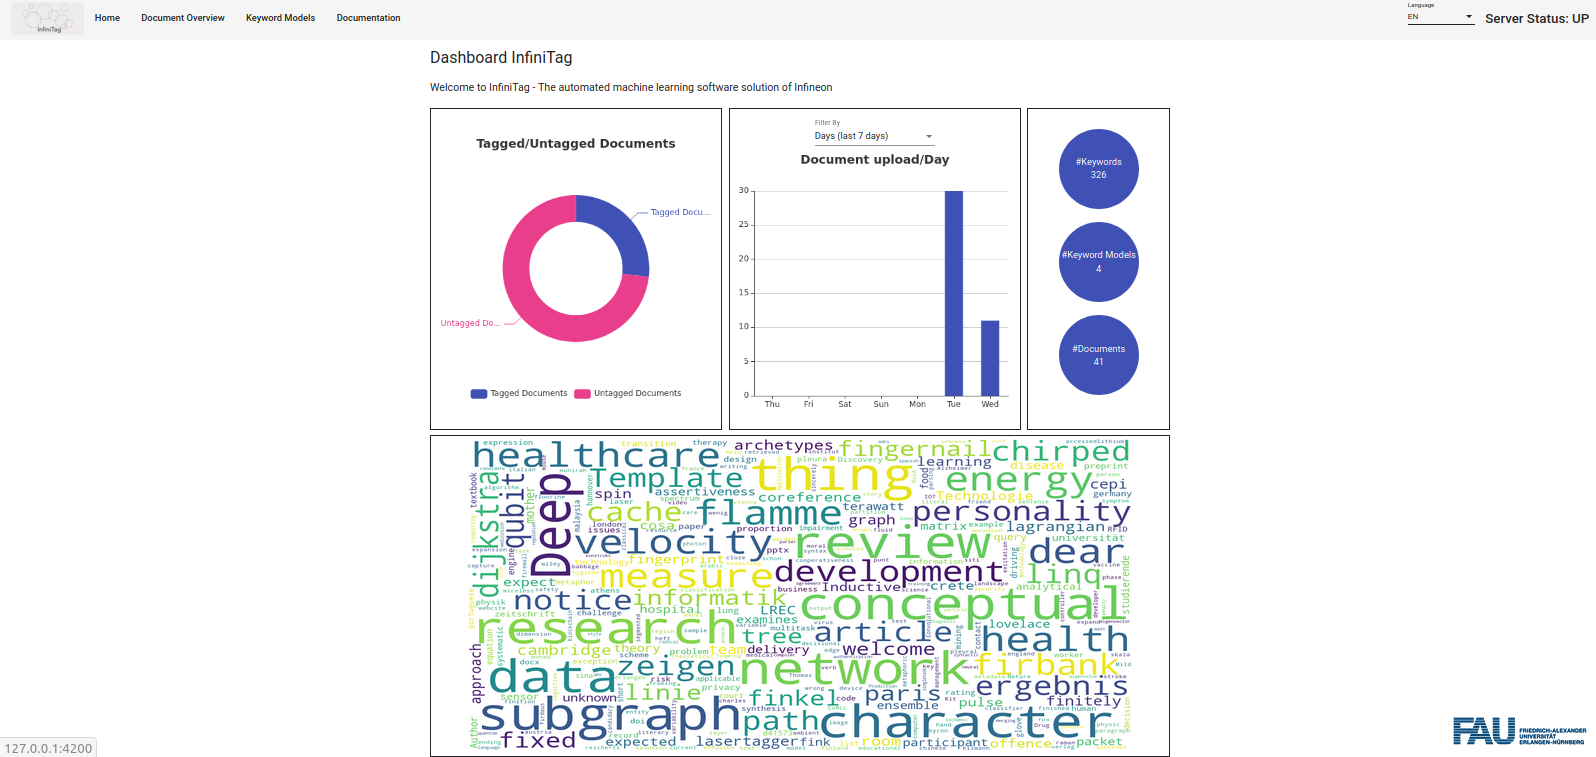
\includegraphics[scale=0.25]{img/dashboard.png}
    \caption{The Start page}
    \label{fig:start_page}
\end{figure}


\section{Document Overview} \label{docoverview}

By clicking on the Document Overview tab in the toolbar you can navigate to the page showing you all documents in the database as seen in Figure \ref{fig:doc_overview}.
The files can be sorted by their attributes by clicking on the respective label. At the top of the page is a search bar allowing you to filter files by a search term.
As the default every field in the database gets searched for the entered term, which also includes the documents name and content.
If you only want to search for specific tags you can press the Search keywords only checkbox.
Our search algorithm translates the search term, which allows you to find documents with either the english and the german word through a single search.
In addition to that you can filter documents by their last edited timestamp by clicking on the Search By Date Range field.


You can upload more files by dragging them into the designated area marked blue or open a file dialog by clicking on it.
A dialog will open allowing you the upload status as well as giving you an option to cancel the upload.


Keywords can be added to documents by clicking on the + sign in the MyKeywords column and can be deleted by pressing the x next to the keyword.
If you wish to add/delete multiple keywords to/from multiple documents at once, you can do so by selecting the Tagging tab.
A checkbox will become visible next to each document and you can enter multiple keywords into the field titled Search Keywords....
Then the selected keywords can be applied or deleted by pressing the respective button.


In the Tagging tab you can use our automated tagging solution, too. We provide two ways to automatically tag your documents. They can be choosen by selecting them from the drop down menu on the right.
The first one tags documents by utilising something we call keyword models. Keyword models will explained in detail later in the Section \ref{kwms}.
The second method is completly automated. You only need to select the documents or click the Apply to all documents button and type in the amount of clusters and keywords you want.
If you are unsure about the number of clusters you want, we also have an option to compute a optimal number, but this option is very runtime intensive, so use it with caution.
The result of all tagging methods can be seen in Figure \ref{fig:applied_kw}. Notice how the keywords are color coded indicating by which method they were created. You can also see their origin by hovering over them.


If you want to download a document you can do that by clicking on the documents File Name or you can download multiple files at once by navigating to the Download/Delete tab.
If you download a couple of files at once, they are combined into a zip file for your convenience. In this tab you can also delete files from the database if you don't need them anymore.

\begin{figure}
    \centering
    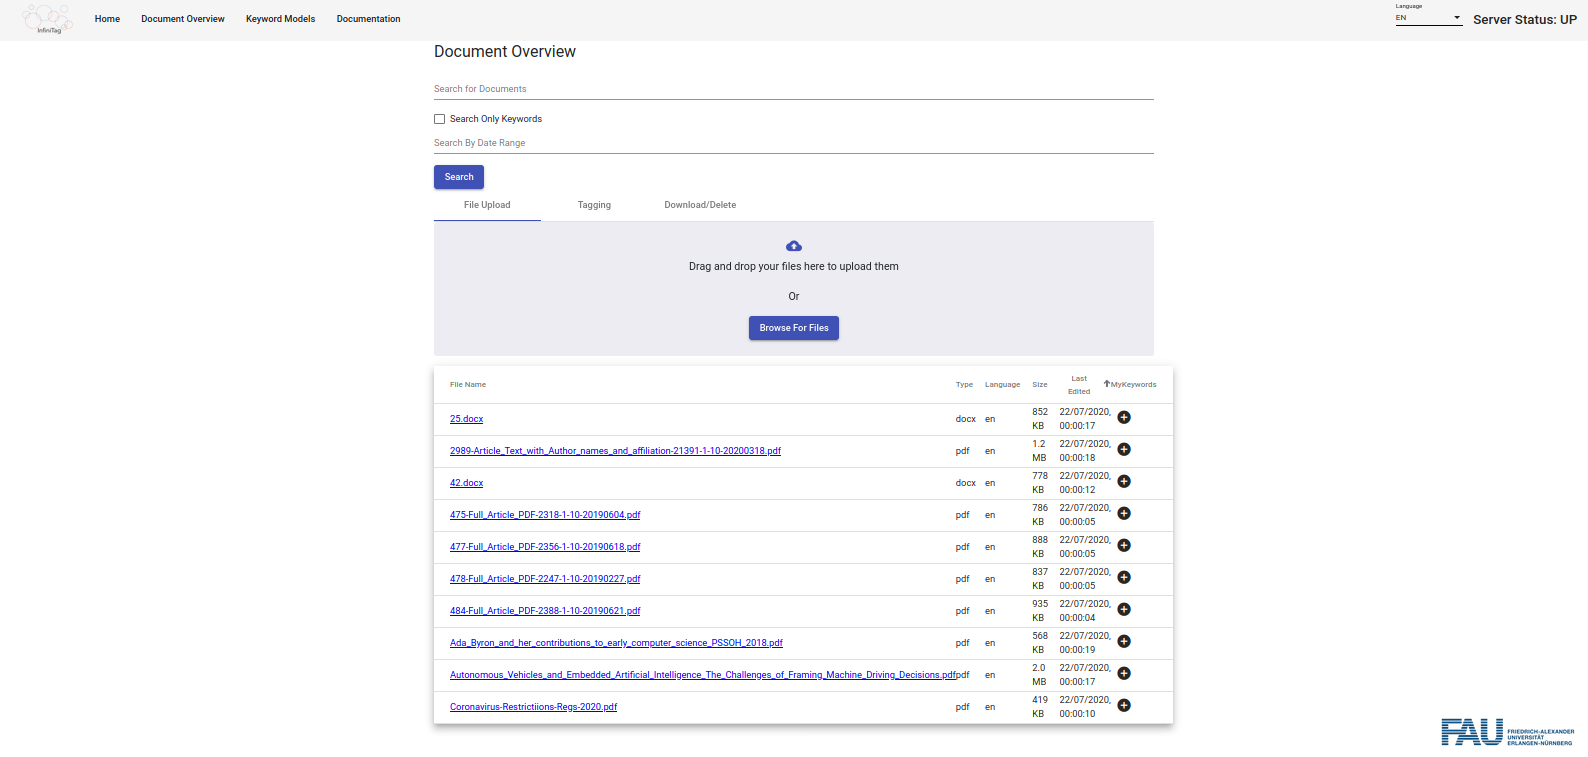
\includegraphics[scale=0.25]{img/doc1.png}
    \caption{The Document Overview}
    \label{fig:doc_overview}
\end{figure}

\begin{figure}
    \centering
    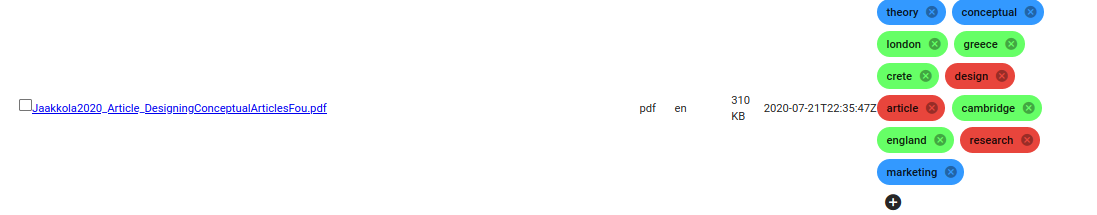
\includegraphics[scale=0.25]{img/applied_kw.png}
    \caption{Keywords applied to a document}
    \label{fig:applied_kw}
\end{figure}

\section{Keyword Models} \label{kwms}
Navigating to the Keywords Models tab will take the user to a page where they can add dimensions and keywords to a keyword model as seen in Figure \ref{fig:key1}.
After adding dimensions/keywords they are first added to their respective uncategorized lists from where they can then be moved to a keyword model on the right by dragging and dropping them into the hierarchy.
Like the name indicates keywords are the actual keywords, which are added to your documents. Dimensions on the other hand don't have an impact, but allow you to create descriptive keyword models.
The root of a keyword model always needs to be a dimension and dimension and keywords need to be alternating as seen in the screenshot.
New keyword models can be created by clicking on the + sign in the middle column. Next to that are buttons for importing and exporting keyword models, allowing you to easyly save, share and load models you generated.

Note that both uncategorized keywords as well as keywords from keyword models appear in the autocomplete list of keywords when adding tags in the document overview.


After designing your keyword model you can apply it using the functionality in the document overview page as descript as in Section \ref{docoverview}.
When applying a model our software checks if the keywords are contained within a document and if found are added as tags to that document. We use lemmatization during this process, allowing you to create compact keyword models.
If you decide to use a model with hierarchy multiple levels deep, our software automatically adds the upper dimensions keywords as well if a lower dimension keyword is found. For example if you apply the cities keyword model show in Figure \ref{fig:key1}
and a document contains one of the cities, the corresponding country keyword gets added as well.
This allows you to tag your documents more efficiently by creating subgroups.

\begin{figure}
    \centering
    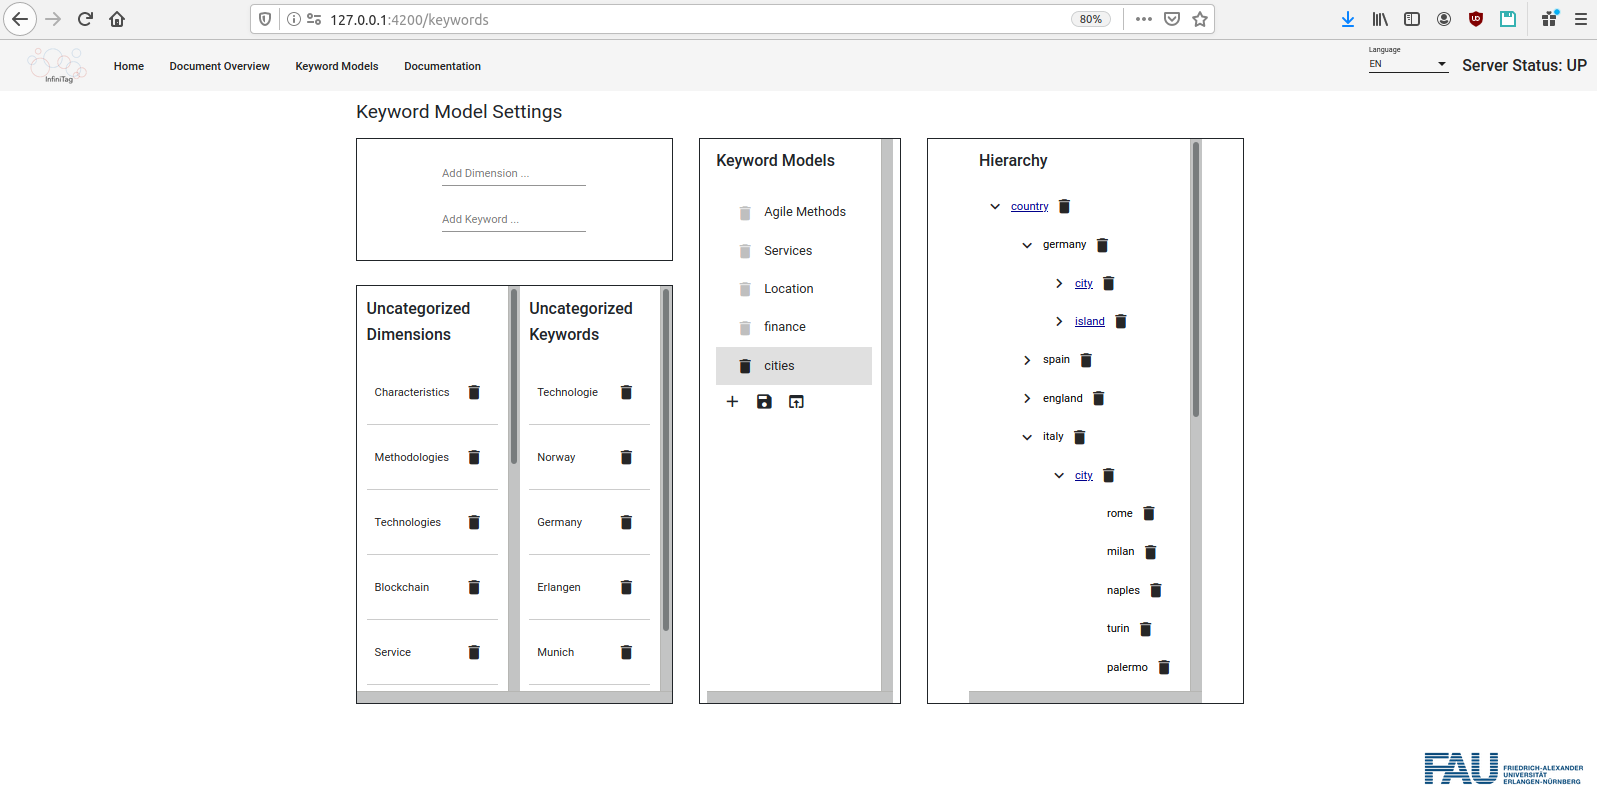
\includegraphics[scale=0.4]{img/key1.png}
    \caption{Maintaining Keywords}
    \label{fig:key1}
\end{figure}

\section{Further Documentation}
Clicking on the \verb|Documentation| link will provide the user with three options as seen in Figure \ref{fig:doc_drop}:

\begin{enumerate}
    \item API Documentation. This provides the user with an overview of all API endpoints for the back end, along with the required parameters and expected return results. A partial example can be seen in Figure \ref{fig:apidoc}
    \item Front End Documentation. This is an external link which will show the user the actual code documentation for the front end.
    \item Back End Documentation. This is another external link which will show the code documentation for the server.
\end{enumerate}

\begin{figure}
    \centering
    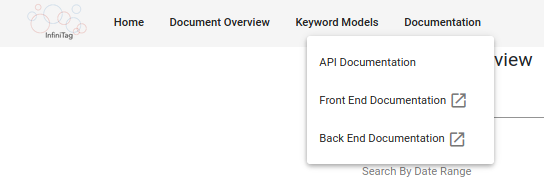
\includegraphics[scale=0.4]{img/doc3.png}
    \caption{Documentation Drop Down}
    \label{fig:doc_drop}
\end{figure}

\begin{figure}
    \centering
    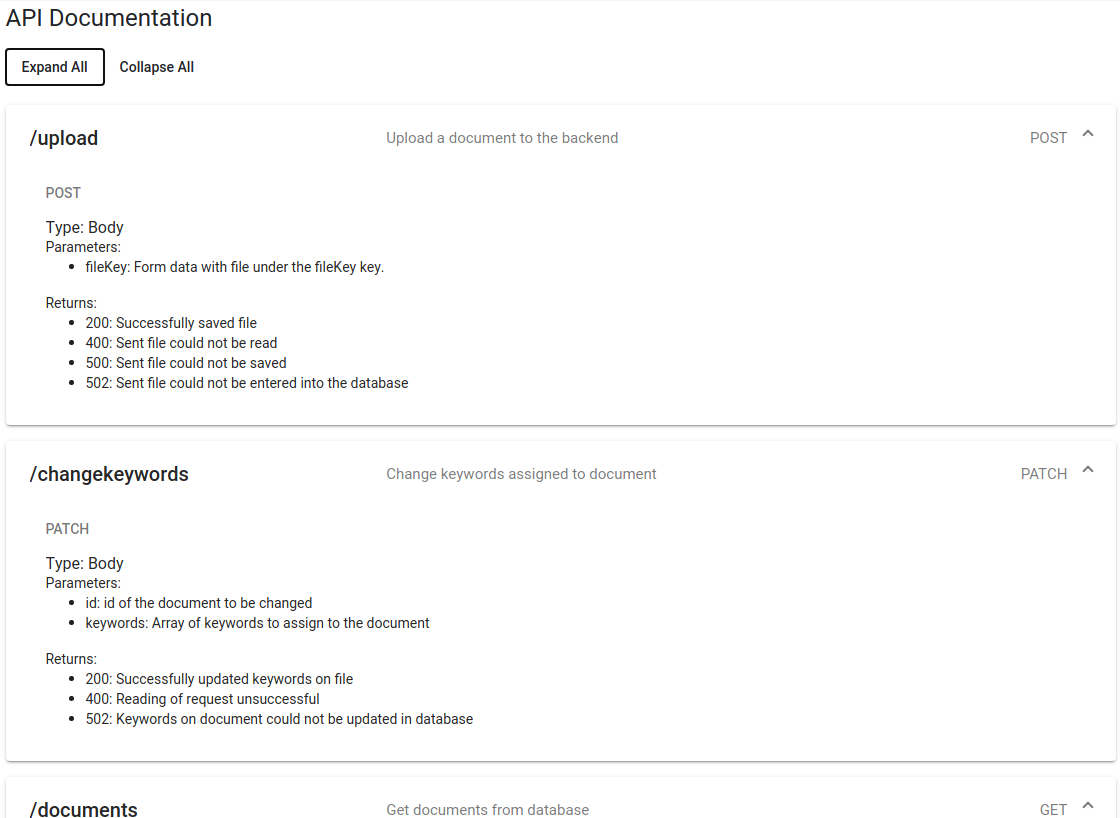
\includegraphics[scale=0.4]{img/api1.png}
    \caption{API Documentation}
    \label{fig:apidoc}
\end{figure}


\section{Utilities}
Important to notice is that the InfiniTag software comes with a utils folder.
Here you can find a tool for crawling an archive site for CC licensed documents. It was used by our developers to create a dataset, which we later decided not to use, but the crawler is still there for completeness.
For further documentation on the crawler you can check out \href{https://github.com/AMOS-5/infinitag/blob/master/docs/crawler/README.md}{README}


\section{License}
InfiniTag Copyright © 2020 AMOS-5
Permission is hereby granted,
free of charge, to any person obtaining a copy of this software and
associated documentation files (the "Software"), to deal in the Software
without restriction, including without limitation the rights to use, copy,
modify, merge, publish, distribute, sublicense, and/or sell copies of the
Software, and to permit persons to whom the Software is furnished to do so,
subject to the following conditions: The above copyright notice and this
permission notice shall be included in all copies or substantial portions
of the Software. THE SOFTWARE IS PROVIDED "AS IS", WITHOUT WARRANTY OF ANY
KIND, EXPRESS OR IMPLIED, INCLUDING BUT NOT LIMITED TO THE WARRANTIES OF
MERCHANTABILITY, FITNESS FOR A PARTICULAR PURPOSE AND NONINFRINGEMENT. IN
NO EVENT SHALL THE AUTHORS OR COPYRIGHT HOLDERS BE LIABLE FOR ANY CLAIM,
DAMAGES OR OTHER LIABILITY, WHETHER IN AN ACTION OF CONTRACT, TORT OR
OTHERWISE, ARISING FROM, OUT OF OR IN CONNECTION WITH THE SOFTWARE OR THE
USE OR OTHER DEALINGS IN THE SOFTWARE.
\end{document}

